\testCom
{3.134}
{
	В схеме (рис. 3.34) ЭДС элемента $\varepsilon$ = 2,0 В, его внутреннее сопротивление $r$ = 9,0 Ом, 		емкость конденсатора $C$ = 10 мкФ, индуктивность катушки $L$ =100 мГн и активное сопротивление $R$ = 	1,0 Ом. В некоторый момент ключ К разомкнули. Найти энергию колебаний в контуре:\\
	а)непосредственно после размыкания ключа;\\
	б)через $t$ = 0,30 с после размыкания ключа.
}
{%Дано
	$\varepsilon$ = 2,0 В\\
	$r$ = 9,0 Ом\\
	$C$ = 10 мкФ\\
	$L$ =100 мГн\\
	$R$ = 1,0 Ом\\
}
{%Найти
	$E(t)$ - ?
}
{%Решение
	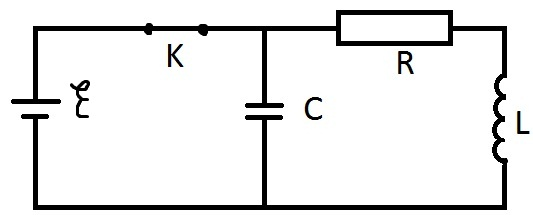
\includegraphics[height=30mm]{3_134.jpg}\\
	${I}_{R}=\frac{\varepsilon}{R+r}$\\
	${U}_{C}={I}_{R}R$\\
	${E}_{0}=\frac{C{U}_{C}^2}{2}+\frac{L{I}_{R}^2}{2}$\\
	${E}_{0}=\frac{C({I}_{R}R)^2}{2}+\frac{L{I}_{R}^2}{2}$\\
	${E}_{0}=\frac{1}{2}{I}_{R}^2(CR^2+L)$\\

	${E}_{0}=\frac{1}{2}(\frac{\varepsilon}{R+r})^2 (CR^2 + L)$\\

	${\omega}_{0}=\frac{2\pi}{T}; T=\sqrt{LC}$\\
	$\sigma=\frac{R}{2L}$ - коэффициент затухания\\  
	$W={W}_{0}e^{-\frac{R}{L}t} \cos\omega t$ - энергия\\
	$E(t) = {E}_{0}e^{-2\sigma t} \cos\omega t$\\
	длинный вывод формулы энергии\\
}

